%\begin{savequote}[75mm]
%Nulla facilisi. In vel sem. Morbi id urna in diam dignissim feugiat. %Proin molestie tortor eu velit. Aliquam erat volutpat. Nullam ultrices, diam tempus vulputate egestas, eros pede varius leo.
%\qauthor{Quoteauthor Lastname}
%\end{savequote}
\chapter{Introduction}

We are in a crisis of understanding. The magnitude and complexity of the climate crisis and its many related crises demand that we change the tools and methods we use to think. This thesis proposes a novel framework for activating large texts, particularly in the critical domain of climate resilience. In this thesis, I propose a response to the climate crisis that builds on the ways we reason with symbols and graphs as a means to accelerate interdisciplinary knowledge work. 

The climate crisis is accelerating which imposes a shrinking timeline for innovating ways to face it. Furthermore, while we may need to create new tools and methods, we may already have solutions for climate crisis mitigation that lie unactivated in the silos of research repositories and their marginalia.

My thesis positions itself at this intersection of urgent global need, and emerging technological possibility. In a time in history when time saved in research could mean the survival of innumerable humans and other forms of life, the development of better ways to work with knowledge could hardly be more urgent. 

The core of this thesis are three tools to working with graphs of texts: Semantic Forms, Query Isomorphs, and TCA Workspace. TCA Workspace is a software platform that will accelerate the computational analysis of texts and graphs. It integrates Semantic Forms for three-dimensional modeling of text graphs, Query Isomorphs for topological querying using Persistence Homology, and tools for Symbol-setting, gigamapping, and Systematic Combining. Epistemologically, TCA Workspace functions as a sort of particle accelerator of ideas, where researchers can examine and activate not books, but living webs of thought.
\index[terms]{gigamapping}
\index[terms]{Systematic Combining (SC)}



\section{Background and context}

\subsection{Research Problems and Significance}

Our crisis of understanding demands new solutions, and fast. However, the growing amount of information makes it impossible to consider all data. As Drucker notes, “The expansion of access to any and all stored data that can be repurposed and remediated nearly boggles the mind” \citep[p. 194]{drucker_graphesis_2014}.
\index[people]{Drucker, Johanna}

There is not enough time left in the universe to work through all the information in each discipline and find solutions. We need new tools that help cope with complex information \citep[p. 34]{sevaldson_designing_2022}, and that facilitate conceptual translation between disciplines. Activating large texts in this way would reveal solutions to new issues from what has already been discovered. Paradigm-shifting solutions for climate resilience almost certainly exist, and we must endeavour to find and apply them. Some new knowledge production will be necessary, but solutions may already exist; we may have all we need to solve it, and we may just need to activate the knowledge we already have.
\index[people]{Sevaldson, Birger}

Computational tools can accelerate knowledge work around climate resilience. However, considering the integration of multi-disciplinary approaches required, we must co-inform software engineering skills with the ``imaginative sensibility”  \cite[p. 194]{drucker_graphesis_2014}. Humanistic information design interface \citep[p. 178, 190-191]{drucker_graphesis_2014} must question data as fact, and instead computationally analyze `capta', or the ways information is inherently ``constructed interpretation motivated by a human agenda" \citep[p. 131]{drucker_graphesis_2014}.



\subsection{Research Questions}
\textbf{RQ1}: \textit{What philosophical, mathematical, and computational approaches to textual/graphical analysis can accelerate knowledge work?}

\begin{enumerate}
    \item[\textbf{RQ1.1}] \textit{What forms of spatial information visualization are there, and how can they inform the composition of network graphs?}
    \item[\textbf{RQ1.2}] \textit{How can Computational Analysis of Texts and Graphs (CATG) identify isomorphic semantic structures within large network graphs?}
    \item[\textbf{RQ1.3}] \textit{What methods can reveal the relationships between fundamental ideas in texts, graphs, or Large Language Models (LLMs)?}
    \item[\textbf{RQ1.4}] \textit{Given the semantic versatility of symbols, how can a practice of collaborative symbol-making support knowledge production?}
    \item[\textbf{RQ1.5}] \textit{How can CATG reveal relationships between place and text?}
    \item[\textbf{RQ1.6}] \textit{What strategies can improve university knowledge management to accelerate research?}
    \item[\textbf{RQ1.7}] \textit{What sort of knowledge work software would I want to build to incorporate my various findings and use spatial information visualization to identify isomorphic semantic structures, reveal the relationships between fundamental ideas, build on collaborative symbol-making, reveal relationships between place and text, and improve university knowledge management?}
\end{enumerate}




\subsection{Thesis Statement and Contributions}


\textit{The climate crisis continues to accelerate faster than climate resilience research and operationalization can keep up. Novel approaches for Knowledge Activation can catalyze paradigmatic shifts in Sustainability Transitions (ST).}

\textbf{The main contributions of this thesis are a set of such novel approaches proposed for visuospatial Knowledge Activation (KA) using human-in-the-loop (HITL) Computational Analysis of Texts and Graphs (CATG), Human Analysis of Texts and Graphs (HATG), or both, for the surfacing, synthesis, translation, and production of knowledge:}

\begin{enumerate}
    \item[\textbf{C1}] \textit{Semantic Forms}, a taxonomy of three-dimensional topic model compositions for HITL CATG, HATG, or both.
    \item[\textbf{C2}] \textit{Query Isomorphs} as a means of Topological Capta Analysis (TCA) in HITL CATG using small graph chunks.
    \item[\textbf{C3}] \textit{Ontological Semantic Network Summaries (OSNS)} as a means of revealing ontological relationships between ideas in a given body of research using HITL CATG, HATG, or both.
    \item[\textbf{C4}] \textit{Symbol-setting}, a method for expanding the semiotic range of knowledge production using symbol co-creation in HITL CATG, HATG, or both.
    \item[\textbf{C5}] \textit{Terroir of Text and Graphs (TTG)}, a method of HITL CATG that uses TCA to interpret and reveal semantic relationships between (a) texts and graphs, and (b) the features and systems of ecological place.
    \item[\textbf{C6}] \textit{TCA Researcher Grouping}, a proposal to use TCA for grouping research collaborators more effectively using HITL CATG, HATG, or both; finally,
    \item[\textbf{C7}] \textit{TCA Workspace}, a proposal for a collaborative HITL CATG + HATG platform to:
    \begin{enumerate}
        \item[(a)] house all my thesis contributions (\textit{Semantic Forms}, \textit{Query Isomorphs}, \textit{OSNS}, \textit{Symbol-setting}, \textit{TTG}, and \textit{TCA Researcher Grouping}).
        \item[(b)] facilitate their combined use with Systemic Design methods for visuospatial reasoning discovered through my literature review, such as gigamapping \citep{sevaldson_giga-mapping_2011}, \citep[p.~26]{sevaldson_designing_2022} and Systematic Combining \citep[p.~554]{dubois_systematic_2002}, \citep{kjode_entanglement_2024}.
    \end{enumerate}
\end{enumerate}

\index[terms]{gigamapping}
\index[terms]{Systematic Combining (SC)}

\FloatBarrier
\begin{figure}[h]
    \centering
    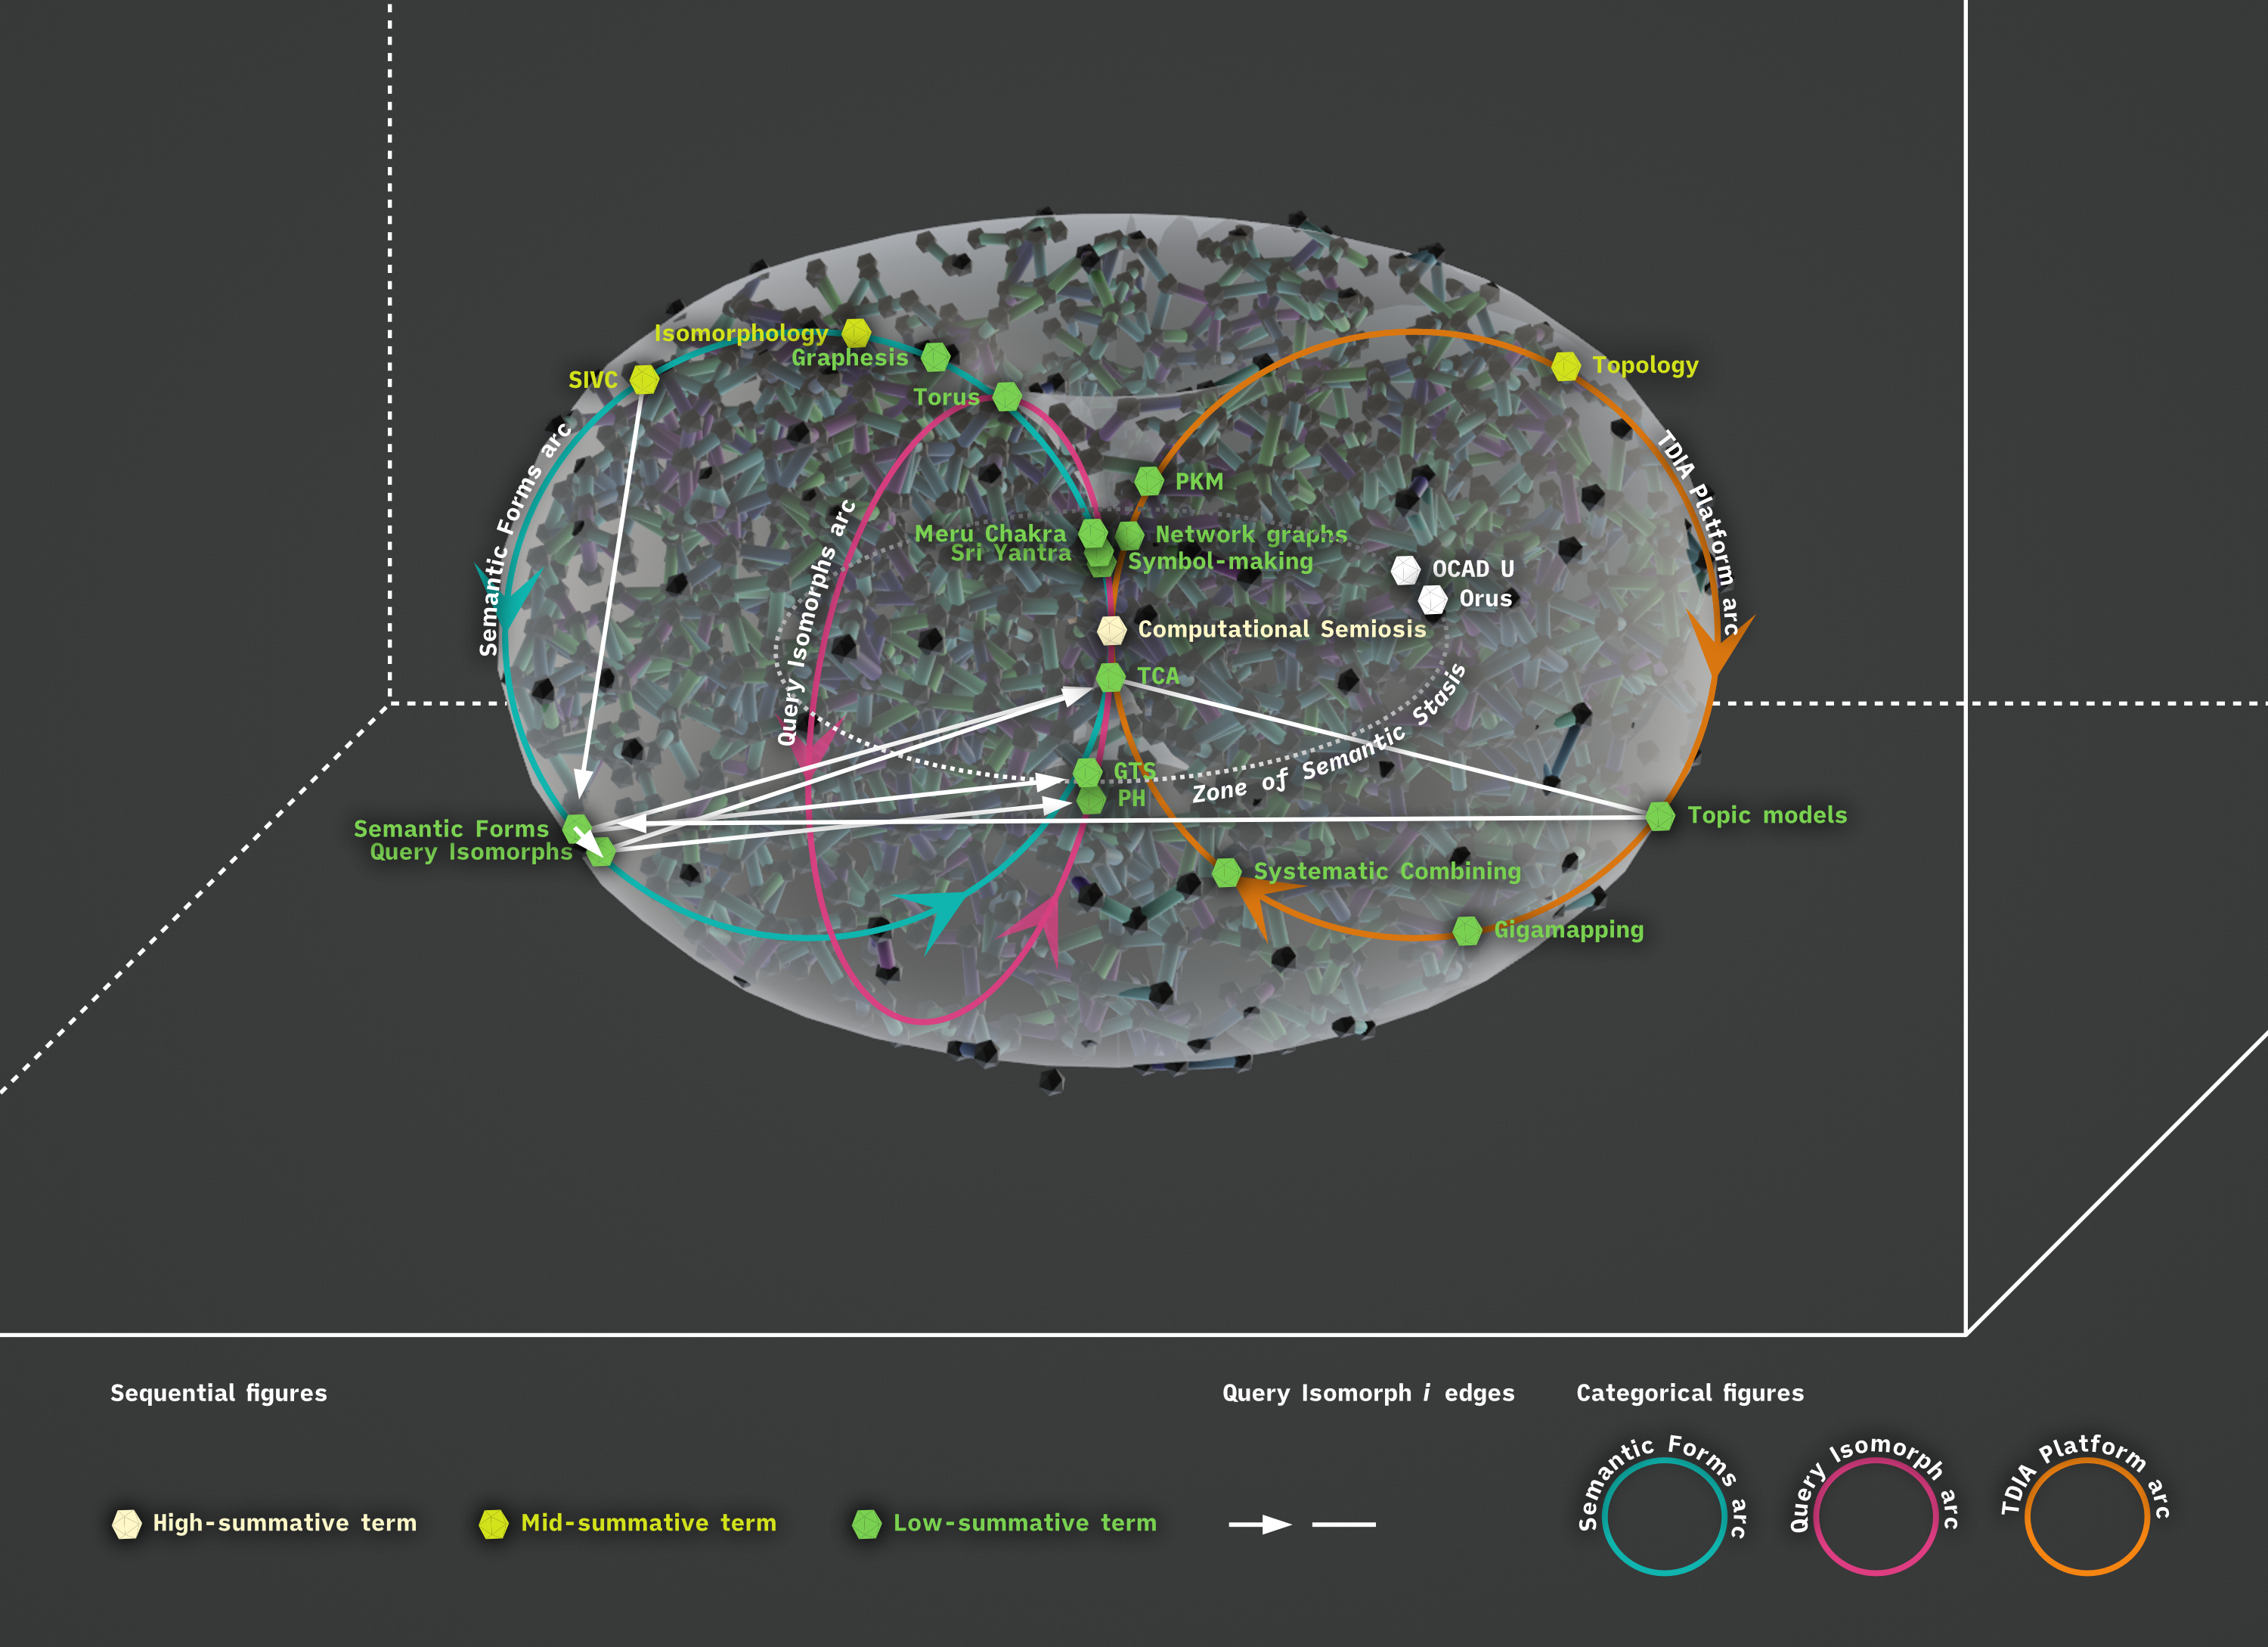
\includegraphics[width=\textwidth]{figures/5.16.HT1.png}
    \caption[Preview of illustrations]{{\textbf Preview of illustrations.} Horn Torus Semantic Form about Query Isomorph \textit{i}. Render of how TCA Workspace would render a Query Isomorph about this thesis located in a Horn Torus Semantic Form network graph.}
    \label{f5.16.HT1}
\end{figure}
\index[terms]{Sri Yantra}
\index[terms]{Meru Chakra}
\index[terms]{gigamapping}
\index[terms]{Systematic Combining (SC)}
\index[terms]{Horn Torus Semantic Form}

\FloatBarrier
\clearpage


\subsection{My prior work}
In the OCAD U School of Graduate Studies I am working across the programs for Digital Futures Program and Strategic Foresight and Innovation. As a brand designer, symbols and their connection to learning have been a longstanding interest of mine which sparked a strong desire for me to understand learning how to learn in a deeper way. This exploration led me to ways symbols could be represented in three-dimensional and multidimensional space over time. A significant breakthrough for me was understanding the two-dimensional Sri Yantra \citep[p. 2]{buhnemann_mandalas_2003} alongside the three-dimensional Meru Chakra \citep[p. 31]{buhnemann_mandalas_2003}. This merging of theology, technology, and psychology inspired me to explore multidimensional forms as interfaces for capturing and examining complex ideas. I aimed to accelerate research, especially in climate resilience.
\index[terms]{Sri Yantra}
\index[terms]{Meru Chakra}


\section{How this thesis is organized}
Leading out from this introduction, this thesis will move from literature review, methodology and methods, preliminary work, visuospatial models derived from theory, methodological and theoretical proposals derived from visuospatial models, a reflection on the literature review, a discussion of my contributions, and a conclusive call to action. 

In Chapter 2, Literature Review, I offer a mixed methods and scoping review. In sections 1-6 I frame my thesis with its urgencies and theoretical context. First, I name the high stakes of the climate crisis and its sociopolitics, the cognitive toll of climate complexity, the role of design as a mediator for complexity. I then retrace the post-structuralist approaches to language and humanistic design that inform my thesis. I then discuss John F. Sowa's work as an example of how language and reasoning are interpreted using computational graphing. Next, I discuss network graphs, their three- and higher-dimensional applications, and my entry point through Vedic symbol culture. Next, I discuss the multi-mathematical and computational approaches that facilitate the analysis of complex network graphs including AI. In section 7 I present a review that disambiguates the various modes of activating knowledge: Knowledge Surfacing, Synthesis, Translation, and Production (KSSTP). In section 8 I present the ways design cuts across these various modes of Knowledge Activation.
\index[people]{Sowa, John F.}

In Chapter 3, Methodology and methods, I present how my work works within the Research-Creation and Critical Systems Methodologies. Here I present my methods, sampling strategy, analytical approaches including Systematic Combining, and Meta-Systematic Combining. 
\index[terms]{Systematic Combining (SC)}

In Chapter 4, Preliminary making, I present my art, design, and code experiments in point plot composition, topic models, and Small Language Models. 

In Chapter 5, From theory to visuospatial models, I present Semantic Forms, Query Isomorphs, and the ways they work together. Next I trace how Systemic Design methods make excellent candidates for applying Semantic Forms and Query Isomorphs through computational application in the Topological Capta Analysis Workspace.

In Chapter 6, From visuospatial models to theory and method, I present Ontological Semantic Network Summaries (OSNS), Symbol-setting, Terroir of Text and Graphs, and TCA Researcher Grouping. 

In Chapter 7, Reflection on my literature review, I present a formulaic expression of Knowledge Activation's diverse modes, and reflections on topology, Personal Knowledge Management, and AI. Next, I present a sensorially diversifying discussion of the word graphesis. Next, I offer an antioppressive critique of the terms blind-spot and stakeholders. To sum up my reflection I conclude with an identification of research gaps I discovered. 

In Chapter 8, Discussion of contributions, I propose implications of realizing Semantic Forms and Query Isomorphs as a software platform. 

In Chapter 9, Conclusion, I retrace the core problems I faced with research questions, and the contributions that emerged. 